\section{Results}\label{study1-results}

Over the week, teams created 1805 entities and 1529 relationships in
total. The number of entities teams created ranged from 24 to 223 ($M=82,
SD=39.9$), and the number of relationships ranged from 7 to 237 ($M=69.5,
SD=51.0$), showing a large variety. The big range was related to different team data modeling strategy,
which will be discussed in detail later. While teams could work on the project any time, we found three intensive usage sessions from the interaction log: two were in class and one was before the team report deadline, outside of class.

CAnalytics was generally well-received by the students. An overview of
the related survey items (shown in Figure~\ref{fig:survey}) shows that students positively rated all aspects
of the tool except cognitive load, towards which they had a close to neutral feeling, which is understandable as the tool does not necessarily reduce the complexity and load of the task.  % \bvh{provide more detail here, don't just rely on the figure}

\begin{figure}
\centering
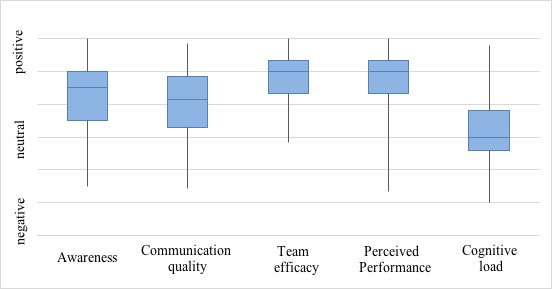
\includegraphics[width=\linewidth]{04-Study_one/img/survey_boxchart.jpg}
\caption{Survey responses (box shows Q1-Q3 and median; ends of whiskers show
maximum and minimum)\label{fig:survey}}
\end{figure}

\subsection{Filtering vs. Accretion}


\begin{figure}
	\centering
	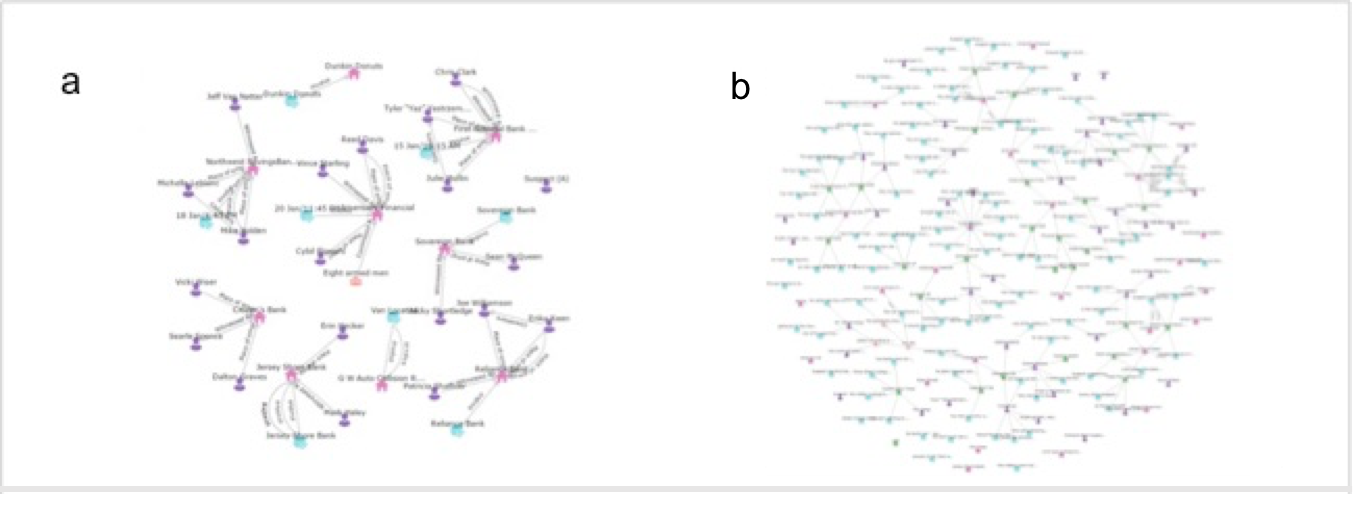
\includegraphics[width=\columnwidth]{./04-Study_one/img/network_accretion_filter.png}
	\caption{Network artifact comparison: filtering (a)
		vs.~accretion (b) \label{fig:network_accretion}}
\end{figure}

In examining participants' created data objects,
we noted a distinction between filtering and accretion
strategies, similar to what was reported in the paper prototype study \citep{Carroll2013}. Filtering is selectively modeling of data
and adding to an artifact. Users must decide what information is
relevant, and thus what is to be excluded, as well as what granularity
of information is to model. Filtering requires more team coordination
because teammates must reach a common ground of the current problem as
well as information needed to answer the problem. Figure~\ref{fig:network_accretion}a is an example of network built with filtering strategy. It only represented key information of robberies.

Accretion is an attempt to comprehensively represent the problem by
adding all information to an artifact. Users extract every fact from the
document, regardless of its immediate relevance to the problem.
Accretion requires less coordination as it is relatively mechanical note-taking. A disadvantage of accretion is that it can be time-consuming
to model all details and the produced artifact could be fairly complex.
An example is Team 108, who modeled
every step the suspects took, which resulted in far more entities (223) than
the average (82) and a more cluttered network view (Figure~\ref{fig:network_accretion}b). This accounted for the large range of entities created. Users also realized the problem. They reflected that they spent too
much time in detail events, and many did not help their analysis at all:

\begin{quote}
	\emph{I felt that after we were done annotating, we hadn't really accomplished
		anything and that we were no closer to solving the case than when we had
		started. In the end it didn't really help that we had annotated the
		data. (P86)}
\end{quote}

\subsection{Situational logic vs. Comparison}

\begin{figure}
	\centering
	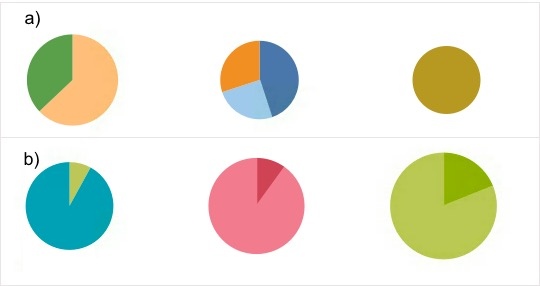
\includegraphics[width=\columnwidth]{04-Study_one/img/labor_division.jpg}
	\caption{Pie charts showing different labor division strategies. Each
		pie chart corresponds to annotations created by one team member. (a) Document-based
		collaboration. Each pie chart shows the documents a team member
		annotated, color coded by document ID. It is clear from the graph that the three team members work on different documents. (b) Entity-based collaboration.
		Each pie chart shows the entity types a team member created, color
		coded by entity types. It is clear that the three team members create different entity types across documents.
	\label{fig:labor_division}}
\end{figure}

We examined the patterns of the annotations teams created. We saw a clear distinction in terms of how teams divided their work in creating annotations. Seven
teams created annotations with a document-based pattern: each teammate focused on their own set of documents and made concrete detailed annotations.
(as shown in Figure~\ref{fig:labor_division}a). Individuals consider the known facts of the current document and seek to identify the cause-effect relationships of this document. We take the term \textit{situational logic} from \citep{Heuer1999} to describe this pattern, in which teams start hypotheses ``with concrete elements of the current situation, rather than with broad generalization that encompasses many similar cases'' (p.32). The team relied on partners to identify and share useful information within their assigned documents. The failing of this
strategy is thus in case an individual fails to identify or convey
evidence in the document, the team may overlook or misunderstand the information
altogether.

Four teams followed a different strategy. Instead of dividing by documents, they divided work by entity types: each individual went through all documents but only focused on and annotated
entities of certain types, e.g.~teammate A only annotated persons and
teammate B annotated locations (as shown in
Figure~\ref{fig:labor_division}b). This is known as a \textit{comparison} strategy \citep{Heuer1999}. When analysts recognize two entities as comparable, they use the known entity to fill gaps in their understanding of the present entity. They build connections between two entities, make analysis of similarities and distinctions. Different from situational logic, comparison interprets the present evidence in the context of precedent elements in other documents, and they could examine entity patterns across multiple documents simultaneously. The challenge is of course to decide whether two entities are truly comparable. There is a tendency to conclude two entities are equivalent simply based on the fact that they are equivalent in some aspects. When individuals fail to convey the assumptions made in the comparison, it could mislead the whole team's reasoning.

The rest (eleven) of the teams did not show specific labor division
patterns. Teammates were reading and annotating
the same document concurrently. Concurrent analysis of a document was challenging if not impossible with paper documents or traditional tools but is possible because the groupware allows them to see new annotations by others in
real time and to build on top of other's annotation. Figure~\ref{fig:close_collaboration}
shows an example where one team worked on the same document simultaneously.
The three team members exhibited high synchronicity in which document to
analyze, which we believe was not by accident. This has the advantage that
teammates are always on the same page and can discuss hypotheses
throughout the analysis process. A problem with this approach is scaling. It demands a lot of individual efforts since each teammate is required to analyze all documents and entities and constantly switch between individual work and collaboration work. As data size increases and analysis time tightens, the team may not afford this approach.


\begin{figure}
	\centering
	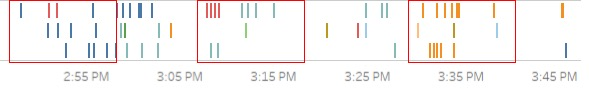
\includegraphics[width=\columnwidth]{04-Study_one/img/close_collaboration.jpg}
	\caption{Graph showing the timeline of one team creating annotations.
		Each row corresponds to one team member. Each bar represents an
		annotation, color coded by document ID. The red blocks highlights the
		periods when teammates worked on the same documents
		simultaneously.\label{fig:close_collaboration}}
\end{figure}



\subsection{Inferential connection vs. Factual discrete}

\begin{figure}
	\centering
	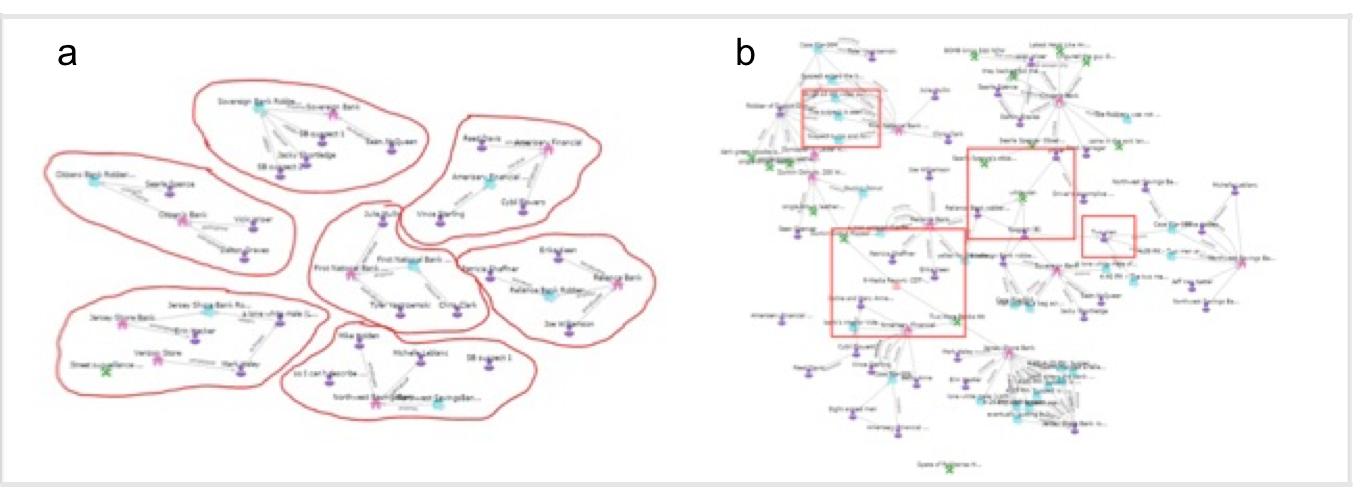
\includegraphics[width=\columnwidth]{04-Study_one/img/network_cluster.png}
	\caption{Network artifact comparison: separate clusters (a)
		vs.~connected clusters (b). The parts highlighted in red squares in (b) are key
		evidence that connects clusters\label{fig:network_cluster}}
\end{figure}

When examining the network artifacts participants created, a clear distinction exists in the shape of clusters. Networks from eight teams consist of discrete clusters
(Figure~\ref{fig:network_cluster}a): Nodes within a cluster are
connected. They are factual entities and relationships extracted from one single robbery case.  Each cluster is self-contained, with no links in between. In contrast, six other teams created networks that consist of connected clusters. Nodes and links within a cluster are similar to ones in the discrete cluster, but these clusters are connected through an
inferential link (Figure~\ref{fig:network_cluster}b, marked in red in the graph).

The differences in network artifacts relate to how teams annotated and represented entities in documents, especially in circumstances of incomplete, ambiguous information. For example, we have the following document snippets:

\begin{quote}
	Case 1: Suspect is shown running down N Atherton and jumping the passenger side of a white van
	
	Case 2: [...] we all watched as the guy ran around the parking lot. I went to the door and saw him jump into a white van of some type
\end{quote}

In both cases, suspects are associated with ``a white van''. Yet with only that information we are not able to conclude the white vans are the same one. That's the \textit{uncertainty} analysts must consider, and must properly represent. We see three types of annotation in team's network artifacts, as shown in Figure~\ref{fig:van}. In figure a, the vans are treated as two separate entities with the same name. It keeps their relationship open to question, yet analysts might have difficulty in identifying this hidden link in later analysis, especially when the network scales. In figure b, analysts merge the two vans into a single entity. This representation makes the connection apparent, yet misses the uncertainty information, which could mislead teammates. We found some teams using the notepad tool in CAnalytics to complement that the link is hypothetical. In figure c, vans are perceived as two entities but connected with a link, which is often labeled with text like ``hypothetical''. 

The three representations reflect different strategies in handling uncertainty. In figure a, analysts are more ``negative'', or conservative, toward uncertainty. They avoid bringing in any hypotheses during the stage of annotation, so as to avoid any bias confirmation in the analysis. In contrast, analysts in figure b are most ``positive'' with uncertainty. If they believe the inferential connection is a high possibility, such representation helps them identify important patterns and make quick decisions. In general, figure c appears to be more reasonable. It represents the connection while preserving the uncertainty, yet requires more annotation efforts. 


\begin{figure}
	\centering
	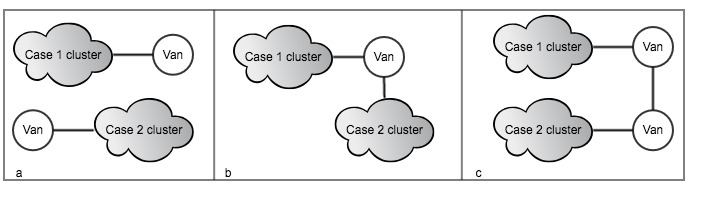
\includegraphics[width=\columnwidth]{04-Study_one/img/van.jpg}
	\caption{Three different representations of uncertainty for entity relationships\label{fig:van}}
\end{figure}

However, it does not mean these teams believe these cases are irrelevant. In fact, these teams still discussed connections between robberies in their report.
It turned out that these teams documented possible relationships in the notepad tool in the form of free text, separate from the network graph. That is, these teams distinguished information content and synthesized them in different artifacts.

%\bvh{how about this - same comment, outline what it means in a sentence and then tie them together like you do in the next sentence.}

By comparing these two types of networks, we found that links within a cluster were typically
\emph{factual} relationships modeled from raw documents (e.g.~a white van was
witnessed at a location), and links between clusters were often
\emph{inferences} beyond literally documented (e.g.~a white van at location A
is the same van witnessed at location B). Teams creating separate
clusters represented only facts in the network and held evidence of
uncertainty in a separate artifact. One advantage of distinguishing
facts and inferences is that teams can always be aware of assumptions made when
making a conclusion. And since all inferences are held in one place,
teams are forced to confront them and review their uncertainty
iteratively in the process. However, the strategy also adds difficulty
to analysis as analysts may overlook or fail to combine evidence
scattered in different artifacts.

% place table simply for paper layout
% % Please add the following required packages to your document preamble:
% \usepackage[table,xcdraw]{xcolor}
% If you use beamer only pass "xcolor=table" option, i.e. \documentclass[xcolor=table]{beamer}
% \usepackage[normalem]{ulem}
% \useunder{\uline}{\ul}{}
\begin{table*}[]
\centering
\caption{Subject feedback of awareness aspects}
\small
\label{tab:awareness}
\begin{tabular}{p{3cm}p{14cm}}
\rowcolor[HTML]{9B9B9B}
\multicolumn{1}{c}{\cellcolor[HTML]{9B9B9B}\textbf{Element}}                           & \multicolumn{1}{c}{\cellcolor[HTML]{9B9B9B}\textbf{Example}}                                                                                                                                                                                                                                                                                                                                 \\
\rowcolor[HTML]{C0C0C0}
\begin{tabular}[c]{@{}l@{}}Social awareness\\ \emph{who is present?}\end{tabular}             & CAnalytics helped me stay aware,of my teammates activities because I could see who was logged on in the top,right corner (P123)                                                                                                                                                                                                                                                              \\
\rowcolor[HTML]{EFEFEF}
\begin{tabular}[c]{@{}l@{}}History awareness\\ \emph{Who has done what?}\end{tabular}         & The way you are able to view when and where your teammate made or updated annotations/information was the key to staying aware of what your team has done. It is a great tool in respects to that. For example, I was able to view the changes my team made while I was not using the CAnalytics tool at the same time they were using the history tab. (P171)                               \\
\rowcolor[HTML]{9B9B9B}
\begin{tabular}[c]{@{}l@{}}Information awareness\\ \emph{What is being changed?}\end{tabular} & CAnalyitics was very helpful in keeping us updated on what was being changed/noted/amended by whom and when. This was very beneficial for staying on the same page and knowing what changes were being made so no one individual was out of the loop. (P157)                                                                                                                                 \\
\rowcolor[HTML]{EFEFEF}
\begin{tabular}[c]{@{}l@{}}Action awareness\\ \emph{Who is doing what?}\end{tabular}          & I liked how you could always see what your teammate were viewing on the website. For example I was working on the bluf when my teammates were working on the network part of the program. If I were to come across a piece of information that I thought might be helpful to them I would just tell them. My teammates did the same thing in return. (P51)                                   \\
\rowcolor[HTML]{C0C0C0}
\begin{tabular}[c]{@{}l@{}}Intention awareness\\ \emph{Who is going to do what?}\end{tabular} & CAnalytics showed what tab {[}tool{]} my teammates were working on which helped me be aware of what they were working on. For example, if I saw that one of my teammates was on the network tab, I knew that they were attempting to connect the information that was relevant to one another.,I would then be able to mention any new findings I had that could influence their work (P160)
\end{tabular}
\end{table*}



On the contrary, in connected-cluster networks, facts and inferences overlaid in one artifact together drive the layout of the
network, are better synthesized, and give analysts a clearer picture in one place. Teams may discuss and evaluate the level of uncertainty of inferences to decide whether to add them to the
network. This strategy makes analysis more interactive among teammates:
they need to negotiate, evaluate, and reach consensus on the value and
validity of inferences. However, a problem with mixing facts and inferences is, to some extent teams might forget whether a
link is factual or inferred, and ask whether conclusion derived
from the visualization can be trusted under uncertainty.


\subsection{Interleaving data annotation and analysis}\label{interleaving-data-annotation-and-data-analysis}

%\bvh{you need the reason why this is interesting...i.e. evidence of these behaviors shows that the tool was used collaboratively}

%\bvh{also what exactly do you mean by interleaving ... you should probably give an example or something??? maybe not, up to you}

We examined the pattern of data modeling and analysis first by
qualitatively looking at a visualization of the entire interaction log
(e.g.~Figure~\ref{fig:interleaving}a shows one team's interaction). All teams
worked intensively on data modeling as they started off the project.
This was the phase when teams were getting themselves familiar with the
documents and made initial annotation input into CAnalytics. Starting from a certain
time point, all teams started analysis on visualizations,
followed by frequent transitions between data modeling and analysis. 11
teams started data analysis in the first usage session, while the other
11 teams had this transition in the second usage session. On average,
the transitions occurred in 47.6 minutes after the project began. The earliest transition occurred in 14 minutes after the team started the project, and the last team
had the transition around 104 minutes, later in the second session. We
also found performance differences among teams that started analysis
early and those late. Teams that started analysis in session one had
higher performance ($M=8.6$) than teams that started from session two
($M=6.7$), although the difference was not statistically significant.

The fact that participants returned to making annotations after analysis
indicated that they did not wait to start analysis till they had
finished modeling. Indeed, the activity of data modeling and data
analysis were highly interleaved throughout the project (as shown by the interleaving color bar in Figure~\ref{fig:interleaving}a). Participants switched from
one activity to the other activity frequently. The state transition
diagram (Figure~\ref{fig:interleaving}b) demonstrates the interleaving in an aggregated way, in which we
encode the number of transitions as the width of a link. This result
confirms our design expectation that data modeling and analysis should
not be supported as separate staged activities, and that an integrated
environment should streamline the workflow.

\begin{figure*}
\centering
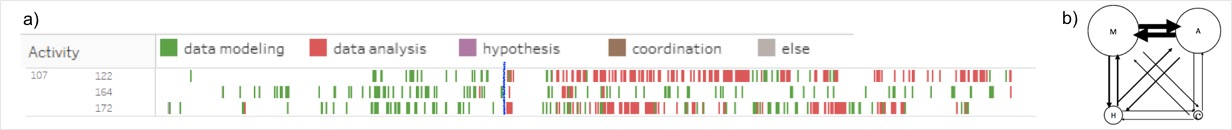
\includegraphics[width=\columnwidth]{./04-Study_one/img/intertwined.jpg}
\caption{(a) Visualization of interaction logs of Team 107. Each row of
colored marks indicates the sequence of top-level activities a
participant performed. (b) State transition diagram of interaction logs of Team 107. Each node is an activity, whose size represents the time spent on it (M: data modeling; A: data analysis; H: hypothesis development; C: coordination); a
link represents a switch from one activity to another, whose width
encodes the number of switches. We see highly frequent transitions between data modeling and data analysis \label{fig:interleaving}}
\end{figure*}




\subsection{Collaboration and
awareness}\label{collaboration-and-awareness}


One recurring theme in the subject feedback we collected was that the
collaboration features were helpful for solving the problem. In the survey
88\% of the students positively rated their
group awareness. Participants appreciated that the tool complemented
traditional analytic tools, describing CAnalytics as Analyst's Notebook with real-time
synchronization features similar to Google Docs, or described it as Google Doc with added visual analytics. To quote one participant,
\emph{``CAnalytics is like an analysts notebook that multiple people
could work on at once {[}\ldots{}and{]} an analysts version of a Google
Doc'' (P65)}.

Participants reflected that they could now contribute simultaneously
without concerns of interference and could
have everything in one place instead of manually sharing documents via a
cloud service.

\begin{quote}
\emph{It was much easier to coordinate as a team with CAnalytics because we
could all work on the same system at the same time. Without CAnalytics,
we were forced to do the work separately and compile all the work onto
one system after we had finished. (P156)}
\end{quote}

Students also reported that being able to see teammate's status made the
task more motivating and engaging:

\begin{quote}
\emph{During class I wasn't sure if my teammates were doing work for that
class or another thing but then seeing their dot {[}tool indicator{]}
switch between applications on the software and updates pop up on my
screen I knew they were doing work for 231. (P141)}
\end{quote}

\begin{quote}
\emph{The fact that you can see what other teammates are doing and they can
see what you are doing creates a sense of accountability in terms of
separating the workload. (P51)}
\end{quote}

The motivating effect of awareness might account for, at least partially,
the fact that teams were participating equally. We measured the equality of
participation in terms of the number of created entities and time spent on
CAnalytics. We refer to Olson \cite{Olson2017} in calculating equality: one
minus the variance of proportions times 100 (for better readability). Thus
the score ranges from .67 (when only one person contributes in a three-member
team) to 1.00 (when everyone participated exactly equally), and a higher
score indicates higher balanced participation. The resulted equality of
created entities and time was .96 and .99 on average respectively. This
indicates participants contributed fairly evenly.

Another repeated theme was the awareness features helped assure all teammates were executing
the team plan. Participants reflected on their experience that a common
team breakdown was a misunderstanding of the team plan, and that they did
not realize the misunderstanding until everyone had spent significant efforts
finishing their ``perceived'' job. CAnalytics made plan execution assured
because they could always see where teammates were working and what they
were generating; and if anything unexpected happened, they could communicate
immediately rather than at the end of the project.

Participants reported many other instances of awareness they realized
using CAnalytics. We categorized them based on the element of awareness,
or the essential problem of awareness of \emph{what}
\citep{Schmidt2002}, into social awareness, information awareness,
action awareness, history awareness, and intention awareness, as shown
in Table~\ref{tab:awareness}.


\begin{table}
	\caption{User reported awareness}
	\label{tab:awareness}
	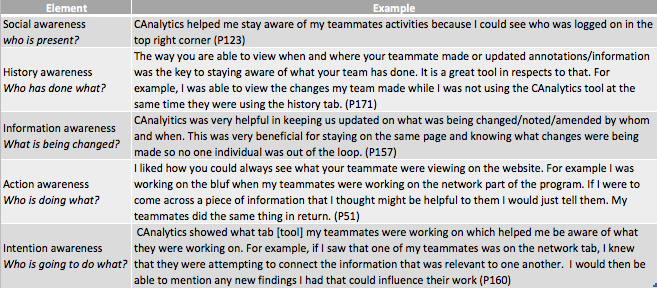
\includegraphics[width=\linewidth]{04-Study_one/img/awareness.png}
\end{table}


When asked what features helped them stay aware of team activities, 28
participants mentioned the tool coordinator, 24 mentioned the
notification system, 19 mentioned the history tool, 14 mentioned the
real-time update of user-generated data, 12 mentioned the collaborative
editor, and 7 mentioned the message tool. Although the number of mentions
does not simply indicate tool usefulness, it suggests users were explicitly aware of these awareness features and appreciated their support.


Students' positive feedback on awareness was further corroborated by
interaction logs. For example, we measured the number of entities
accessed by other collaborators. While data
generated by users is automatically shared, it is up to collaborators
whether to read/edit the shared information or ignore information altogether.
The log showed that on average, 77.6\% of the created entities
were \emph{read} by at least one other teammate. Further, We measured how
many entities were \emph{edited} by collaborators, a phenomenon we argue
requires higher awareness, because the collaborator must not only realize
the creation of the entity, but also understand its content. We
defined \emph{peer editing}, manipulated as the ratio of editing 
entities over editing those created by oneself. We found that all teams
edited collaborator's entity objects, with a peer editing value equal
to .83 ($SD=.45$). The result suggests that teams had little difficulty
accessing and modifying partner's created data objects.

%/bvh{I don't understand this paragraph...what are you trying to say...that they would like to have a shared space?}
One major critique is the lack of support for sharing intermediate analytic
insights. Insight is revealed and contextualized by a specific arrangement of views, e.g.~a reduced data view of interest through filter, a highlighted entity representing the analytic focus, and a clustering layout of network to demonstrate a specific relationship. While teammates share the same data pool, they are likely to have different views of data, and thus different \emph{interpretations}
toward the data. A dynamic view together with its interpretation represents
user's intermediate analytic status. Sharing these insights could inspire team analysis \citep{Gotz2009d}. With CAnalytics
participants complaint that they could not easily make such communications. The team could \emph{``be
looking at the same information but arranged in completely different
ways'' (P131)}.

\subsection{Interaction with team performance}

To systematically evaluate factors that influenced team performance,
we conducted a multiple linear regression between team performance
as the dependent variable and team collaboration characteristics
(i.e.~equality of entities and time respectively, peer editing, number of entities created, shared
entities, switch time from data modeling to analysis) as independent
variables. We treated a team as a system \citep{Henman2003b} and modeled team-level
relationships.
The relationship of individual level variables (e.g.
survey items) could not be simulated with regression directly because data within a team was interdependent. The analysis was performed using \emph{R} \citep{R2016}.

The result is shown in Figure~\ref{fig:regression}. The regression model was found to be statistically significant ($F(5,16)=4.58; p<.01$), with an R squared equal to .59, meaning 59\% of the variability in team performance was explained by the model. Five team-level variables contributed significantly to the prediction of team performance. The model suggested that balanced contribution of entities predicted higher team performance scores ($\beta=45.79, p<.05$), but balanced participation time did not show such effect. More peer editing led to better performance ($\beta=3.89, p<.01$), implying that analysts should be encouraged to model data as a team, and to remodel other's entity objects as needed. Longer elapsed time before a team started analysis (\emph{switch time} in the figure) predicted lower performance ($\beta=-.05, p<.05$), which suggested that teams should shorten the time of pure data modeling and start analysis earlier. A larger number of entities teams created also predicted higher performance ($\beta=.03, p<.05$). This can be interpreted that teams providing sufficient model input did benefit from system support. However, we are not ready to claim more entities are always better because we should also be cautious that entities irrelevant to the team problem bear no value to team analysis, as discussed beforehand. Somewhat surprisingly, the number of shared entities negatively predicted performance ($\beta=-8.99, p<.05$).
%\bvh{hard to understand this sentence...not sure how to rewrite it.}
We considered this might also relate to the issue of entity value: sharing entities without relevance to the team problem leads to reduced team efficiency and creates distraction, which in turn would lead to worse team performance. Another possibility is that teammates may not necessarily access all entities their partners created. The theory of Transactive Memory \citep{Wegner1987} suggests that teammates do not have to know everything in the team but should know ``who knows what''. Individuals specialize in their own field (e.g. one specializes in event analysis while another in social relationship examination) and reach for collaborators when other knowledge is needed. In such cases, common knowledge in shared entities would actually be redundant. Individuals should stay aware of the creator of an entity, but not necessarily the content of every entity.

\begin{figure}
\centering
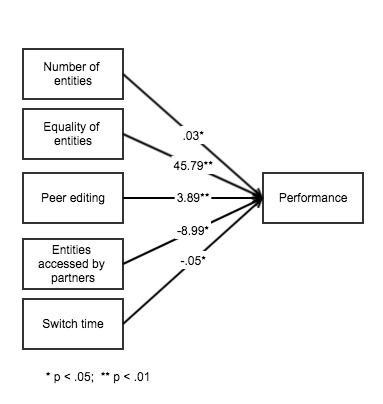
\includegraphics[width=0.6\columnwidth]{04-Study_one/img/team_analysis.jpg}
\caption{The relationship between collaboration characteristics and team performance.\label{fig:regression}}
\end{figure}
